\section{Preliminary: Discrete Flow Matching}
\label{sec:preliminary}
We briefly review the key concepts and notation of discrete flow matching \citep{gat2024discrete,wang2025fudoki} that are used throughout the paper. 
DFM aims to transform a known source distribution $p(x)$ into a target data distribution $q(x)$ over a discrete space. 
We consider $x=(x^1, x^2, \ldots, x^D) \in \mathcal{S}=\mathcal{T}^D$, where $D$ is the number of discrete variables and $\mathcal{T}=[K]=\{1,2,\ldots,K\}$ is the finite alphabet of possible values.

\textbf{Probability Paths}.
Given a \emph{source distribution} \( p(x) \) and a \emph{target distribution} \( q(x) \) on a finite state space \( \mathcal{S} \), DFM defines a family of time-indexed distributions \( \{p_t(x)\}_{t \in [0,1]} \) that smoothly interpolates between \( p \) and \( q \), referred to as \emph{probability paths}.
Each \( p_t(x) \) is constructed as
$p_t(x) \coloneqq \sum_{x_1 \in \mathcal{S}} p_t(x \mid x_1) q(x_1)$,
where the conditional distribution factorizes across dimensions, i.e., $p_t(x \mid x_1) \coloneqq \prod_{i=1}^D p_t(x^i \mid x_1^i)$.
Each term \( p_t(x^i \mid x_1^i) \) interpolates between the base distribution \( p(x^i) \) and a point mass \( \delta_{x_1^i}(x^i) \), i.e., $\delta_{x_1^i}(x^i)=1$ if $x^i=x_1^i$ and $0$ otherwise. 
% We impose the boundary conditions as $p_0(x^i \mid x_1^i) = p(x^i)$ and $\quad p_1(x^i \mid x_1^i) = \delta_{x_1^i}(x^i)$,
% ensuring the path starts from the factorized distribution \( p(x) = \prod_i p(x^i) \) and ends at the target \( q(x) \).
A common choice is the \emph{mixture path} used in~\citep{gat2024discrete,havasi2025edit}, defined by a time-dependent scheduler \( \kappa_t(x_1^i) \in [0, 1] \):
\begin{equation}
p_t(x^i \mid x_1^i) = (1 - \kappa_t(x_1^i)) p(x^i) + \kappa_t(x_1^i) \delta_{x_1^i}(x^i),
\label{eq:mask_probability_path}
\end{equation}
where \( \kappa_0(\cdot) = 0 \) and \( \kappa_1(\cdot) = 1 \). The term $p_t(x^i \mid x_1^i)$ is a \emph{conditional} forward probability path that describes how the state $x^i$ evolves given $x_1^i$. 


\textbf{Probability velocities.}
%
To realize the prescribed probability path $p_{t}(x)$, we use a Continuous-Time Markov Chain (CTMC). Its dynamics are governed by a probability velocity $u_t$, also called the \emph{transition rate}, which describes how the current state $x_t$ moves toward the target state $x_1$ over time. Each token $i$ is updated independently according to
\begin{equation}\label{eq:sample}
x_{t+h}^i \sim \delta_{x_t^i}(\cdot) + h \, u_t^i(\cdot \mid x_t^i, x_1^i),
\end{equation}
where $u_t^i(\cdot \mid x_t^i, x_1^i)$ is the \emph{velocity field}, a conditional rate function that governs the flow of probability from $x_t^i$ to $x_1^i$.
%
Equation (\ref{eq:sample}) can be viewed as a small perturbation of the point mass $\delta_{x_t^i}$ scaled by the step size $h$, which models discrete state transitions in continuous time. The velocity field is central to DFM, which defines the probability-path dynamics and is the main quantity learned during training.

\section{Method}
\begin{wrapfigure}{r}{0.55\textwidth}
    \vspace{-1.2cm}
    \centering
    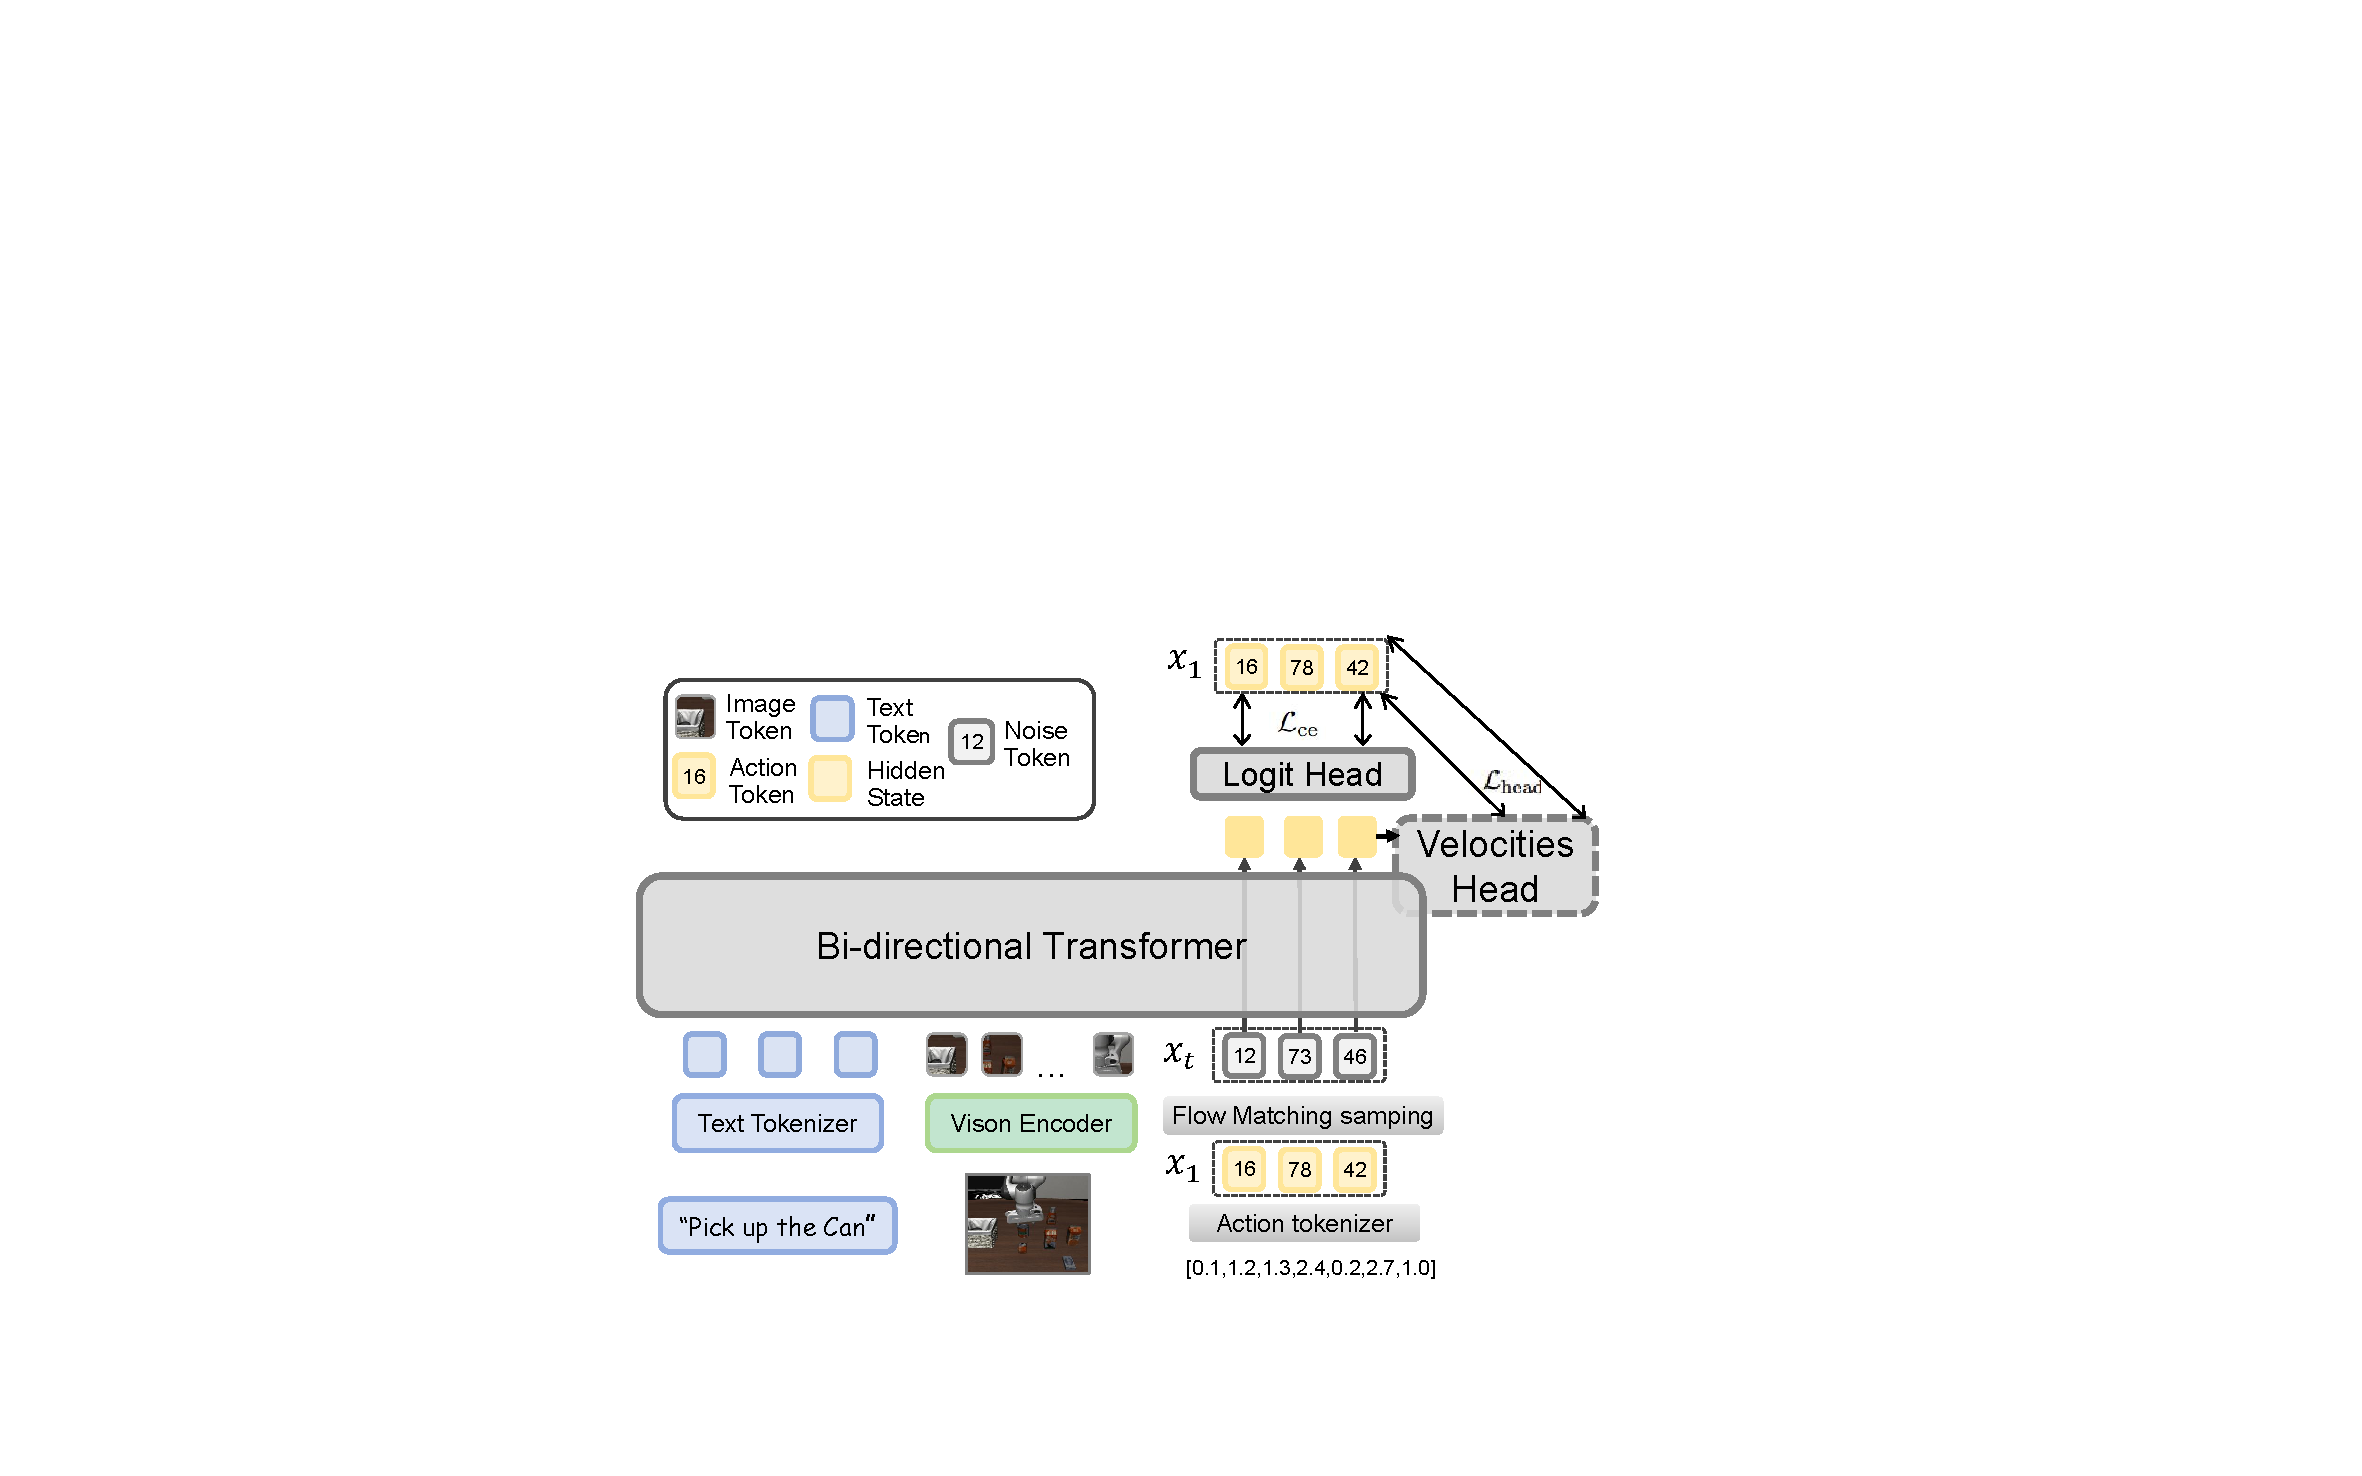
\includegraphics[width=0.99\linewidth]{figure/model.pdf} 
    \caption{Overall architecture of~\method. Given language--vision context and noised action tokens $x_t$, the model predicts clean actions $x_1$ and learns the velocity field via $\mathcal{L}_{\text{ce}}$ or ${L_\text{head}}$.}

     \vspace{-0.5cm}
    \label{fig:model_arch} 
\end{wrapfigure}
This section is organized into four parts. We first introduce the model architecture in Sec.~\ref{subsec:architecture}. We then present two velocity-field constructions: 1) an embedding-guided formulation in Sec.~\ref{sec:Embed_vel} and 2) an auxiliary velocity head formulation in Sec.~\ref{sec:head_vel}. Finally, we describe the two-stage inference procedure in Sec.~\ref{subsec:inference}.
\subsection{Architecture}
\label{subsec:architecture}
% 

As shown in \Cref{fig:model_arch}, 
DFM-VLA follows an architecture similar to UniVLA and adopts a unified discrete-token formulation for language, vision, and action modalities.
Specifically, we tokenize text using the Emu3~\citep{wang2024emu3} tokenizer, and discretize visual observations with a VQ tokenizer~\citep{zheng2022movq} using a compression ratio of 4. Both third-person and wrist-view images are represented as $25\times25=625$ tokens. For action encoding, we discretize continuous actions with FAST~\citep{pertsch2025fast} and further compress action tokens using Byte Pair Encoding (BPE), with an action vocabulary size of 1024. 
To explicitly distinguish modalities, we enclose image and action token spans with boundary markers, i.e., \texttt{boi}/\texttt{eoi} for begin/end of image and \texttt{boa}/\texttt{eoa} for begin/end of action.
In this work, we denote the discretized instruction and observations as $l$, and apply noising and prediction only to the action modality.

\subsection{Action-Embedding-Guided Velocity Modeling}
\label{sec:Embed_vel}

Building on recent advances in discrete flow matching~\citep{gat2024discrete,wang2025fudoki,deng2025uniform}, we parameterize the probability path in a metric-induced form. 
Specifically, let \( d : \mathcal{T} \times \mathcal{T} \to \mathbb{R}_{\geq 0} \) be a distance such that \( d(x^i, x_1^i) = 0 \) if and only if \( x^i = x_1^i \), where \( d(\cdot, \cdot) \) is measured in the action token embedding space. We define the conditional path as
\begin{equation}
p_t(x^i \mid x_1^i) = \mathrm{softmax}\big( -\beta_t \cdot d(x^i, x_1^i) \big),
\label{eq:diffusion-softmax}
\end{equation}
where $\beta_t:[0,1] \to \mathbb{R}_{\ge 0}$ is a monotonic schedule with boundary conditions $\beta_0 = 0$ and $\beta_1 = \infty$. We instantiate it as
\begin{align}\label{eq:beta_t}
\beta_t = c \left(\dfrac{t}{1-t}\right)^\alpha, \qquad t \in [0,1),
\end{align}
where $c>0$ and $\alpha>0$ control how fast probability mass concentrates toward the target token over time. 
% Compared with the mask-based path in Eq.~\ref{eq:mask_probability_path}, 
This formulation preserves semantic neighborhood structure such that tokens closer to $x_1^i$ receive larger probability as $t \to 1$.

Given this prescribed path, we adopt the kinetic-optimal velocity obtained by minimizing transport energy under the flow constraints~\citep{wang2025fudoki,deng2025uniform,luo2025next}:
\begin{equation}
\begin{aligned}
u_t^i(x^i, z \mid x_1) = p_t(x^i \mid x_1^i) \, \dot{\beta}_t \, [ d(z^i, x_1^i) - d(x^i, x_1^i) ]_+
\end{aligned} 
\label{eq:ko-verlocity}
\end{equation}
where $[\cdot]_+ = \max\{\cdot, 0\}$,  $z^i$ is token in the vocabulary $\mathcal{T}$, and $\dot{\beta}_t$ is the derivative of $\beta_t$ w.r.t. $t$. This velocity moves probability mass from $z^i$ to $x^i$ only when $x^i$ is closer to $x_1^i$ than $z^i$, yielding a monotonic refinement process toward the clean target token.

\textbf{Training.}  
Given language--vision context $l$ and corrupted action tokens $x_t$, the model predicts the target action sequence $x_1$ by outputting per-position categorical logits. We optimize the expected cross-entropy:
\begin{equation}
\label{eq:training_loss}
\mathcal{L_\text{ce}} = \mathbb{E}_{t \sim \mathcal{U}[0,1],\, {x}_1, {x}_t}
\left[ -\log p_{1 \mid t}\left( {x}_1 \mid {x}_t, {l}\right) \right].
\end{equation}
where $p_{1|t}^{\theta}(\cdot \mid x_t, l)$ denotes the predicted categorical distribution of the model at each action token position.

\subsection{Modeling Velocities by Additional Head}
\label{sec:head_vel}
% inspire by editflow，我们探索了构建速度场的另一种形式，editflow通过额外的速度头同时建模插入替换以及删除的三种速度场，我们只保留替换操作，因为相对文本而言，动作token的长度设计好的，相对于动作预测任务单独建模动作token的替换速率场就可以，
Drawing inspiration from EditFlow~\citep{havasi2025edit}, which employs additional velocity heads to model three types of edit operations—\emph{insertion}, \emph{replacement}, and \emph{deletion}—we explore an alternative formulation for velocity-field construction. We retain only the \emph{replacement} operation, because the action token sequence length is predefined by our action chunk design and the three operations are fundamentally equivalent under appropriate reformulation~\citep{nguyen2025oneflow,havasi2025edit}. 
% Consequently, for action prediction, modeling only a replacement velocity field is sufficient.
Concretely, given noisy action tokens $x_t$ and context $l$, the backbone first produces hidden states, and the additional velocity head then maps these hidden states to replacement velocities:
\begin{equation}
\label{eq:head-verlocity}
h_t = f_{\theta}(x_t, l), \qquad
u_t^{\theta}(\cdot \mid x_t) = u_t^{\text{head}}(h_t),
\end{equation}
where $f_{\theta}$ denotes the backbone network and $u_t^{\text{head}}$ denotes the velocity prediction head.
\begin{equation}
\small
\mathcal{L_\text{head}}
=
\mathbb{E}_{t \sim \mathcal{U}[0,1],\, {x}_1, {x}_t}
\left[
\sum_{x\neq x_t} u_t^\theta(x\mid x_t)
-
\sum_{i=1}^{N}\mathbf{1}_{[x^i_t\neq x^i_1]}\,
% \frac{\dot{\kappa}_t}{1-\kappa_t}\,
\log u_t^\theta\!\left(x^i\mid x^i_t\right)p_{1 \mid t}\left( {x}^i_1 \mid {x}^i_t, {l}\right)
\right].
\end{equation}
% \begin{equation}
% \mathcal{L_\text{head}}
% =
% \mathbb{E}_{t \sim \mathcal{U}[0,1],\, }
% \left[
% \sum u_t^\theta(x\mid x_t)
% -
% \sum_{i=1}^{N}\mathbf{1}_{[x^i_t\neq x^i_1]}\,
% % \frac{\dot{\kappa}_t}{1-\kappa_t}\,
% \log u_t^\theta\!\left(x^i\mid x^i_t\right)p_{1 \mid t}\left( {x}^i_1 \mid {x}^i_t, {l}\right)
% \right].
% \end{equation}
\noindent Here, \(\mathbf{1}_{[x_t^i \neq x_1^i]}\) is an indicator that equals 1 only when the current token differs from the target token, so the update loss is applied only to positions that still need refinement.
As shown in~\Cref{fig:velocity_field_compare}, the embedding-guided objective (\(\mathcal{L}_{\text{ce}}\)) converges faster and achieves better final performance than the head-based objective (\(\mathcal{L}_{\text{head}}\)). Unless otherwise specified, all experiments use the embedding-guided setting.

\subsection{Inference}
\label{subsec:inference}
\begin{figure*}[t]  
    \centering
    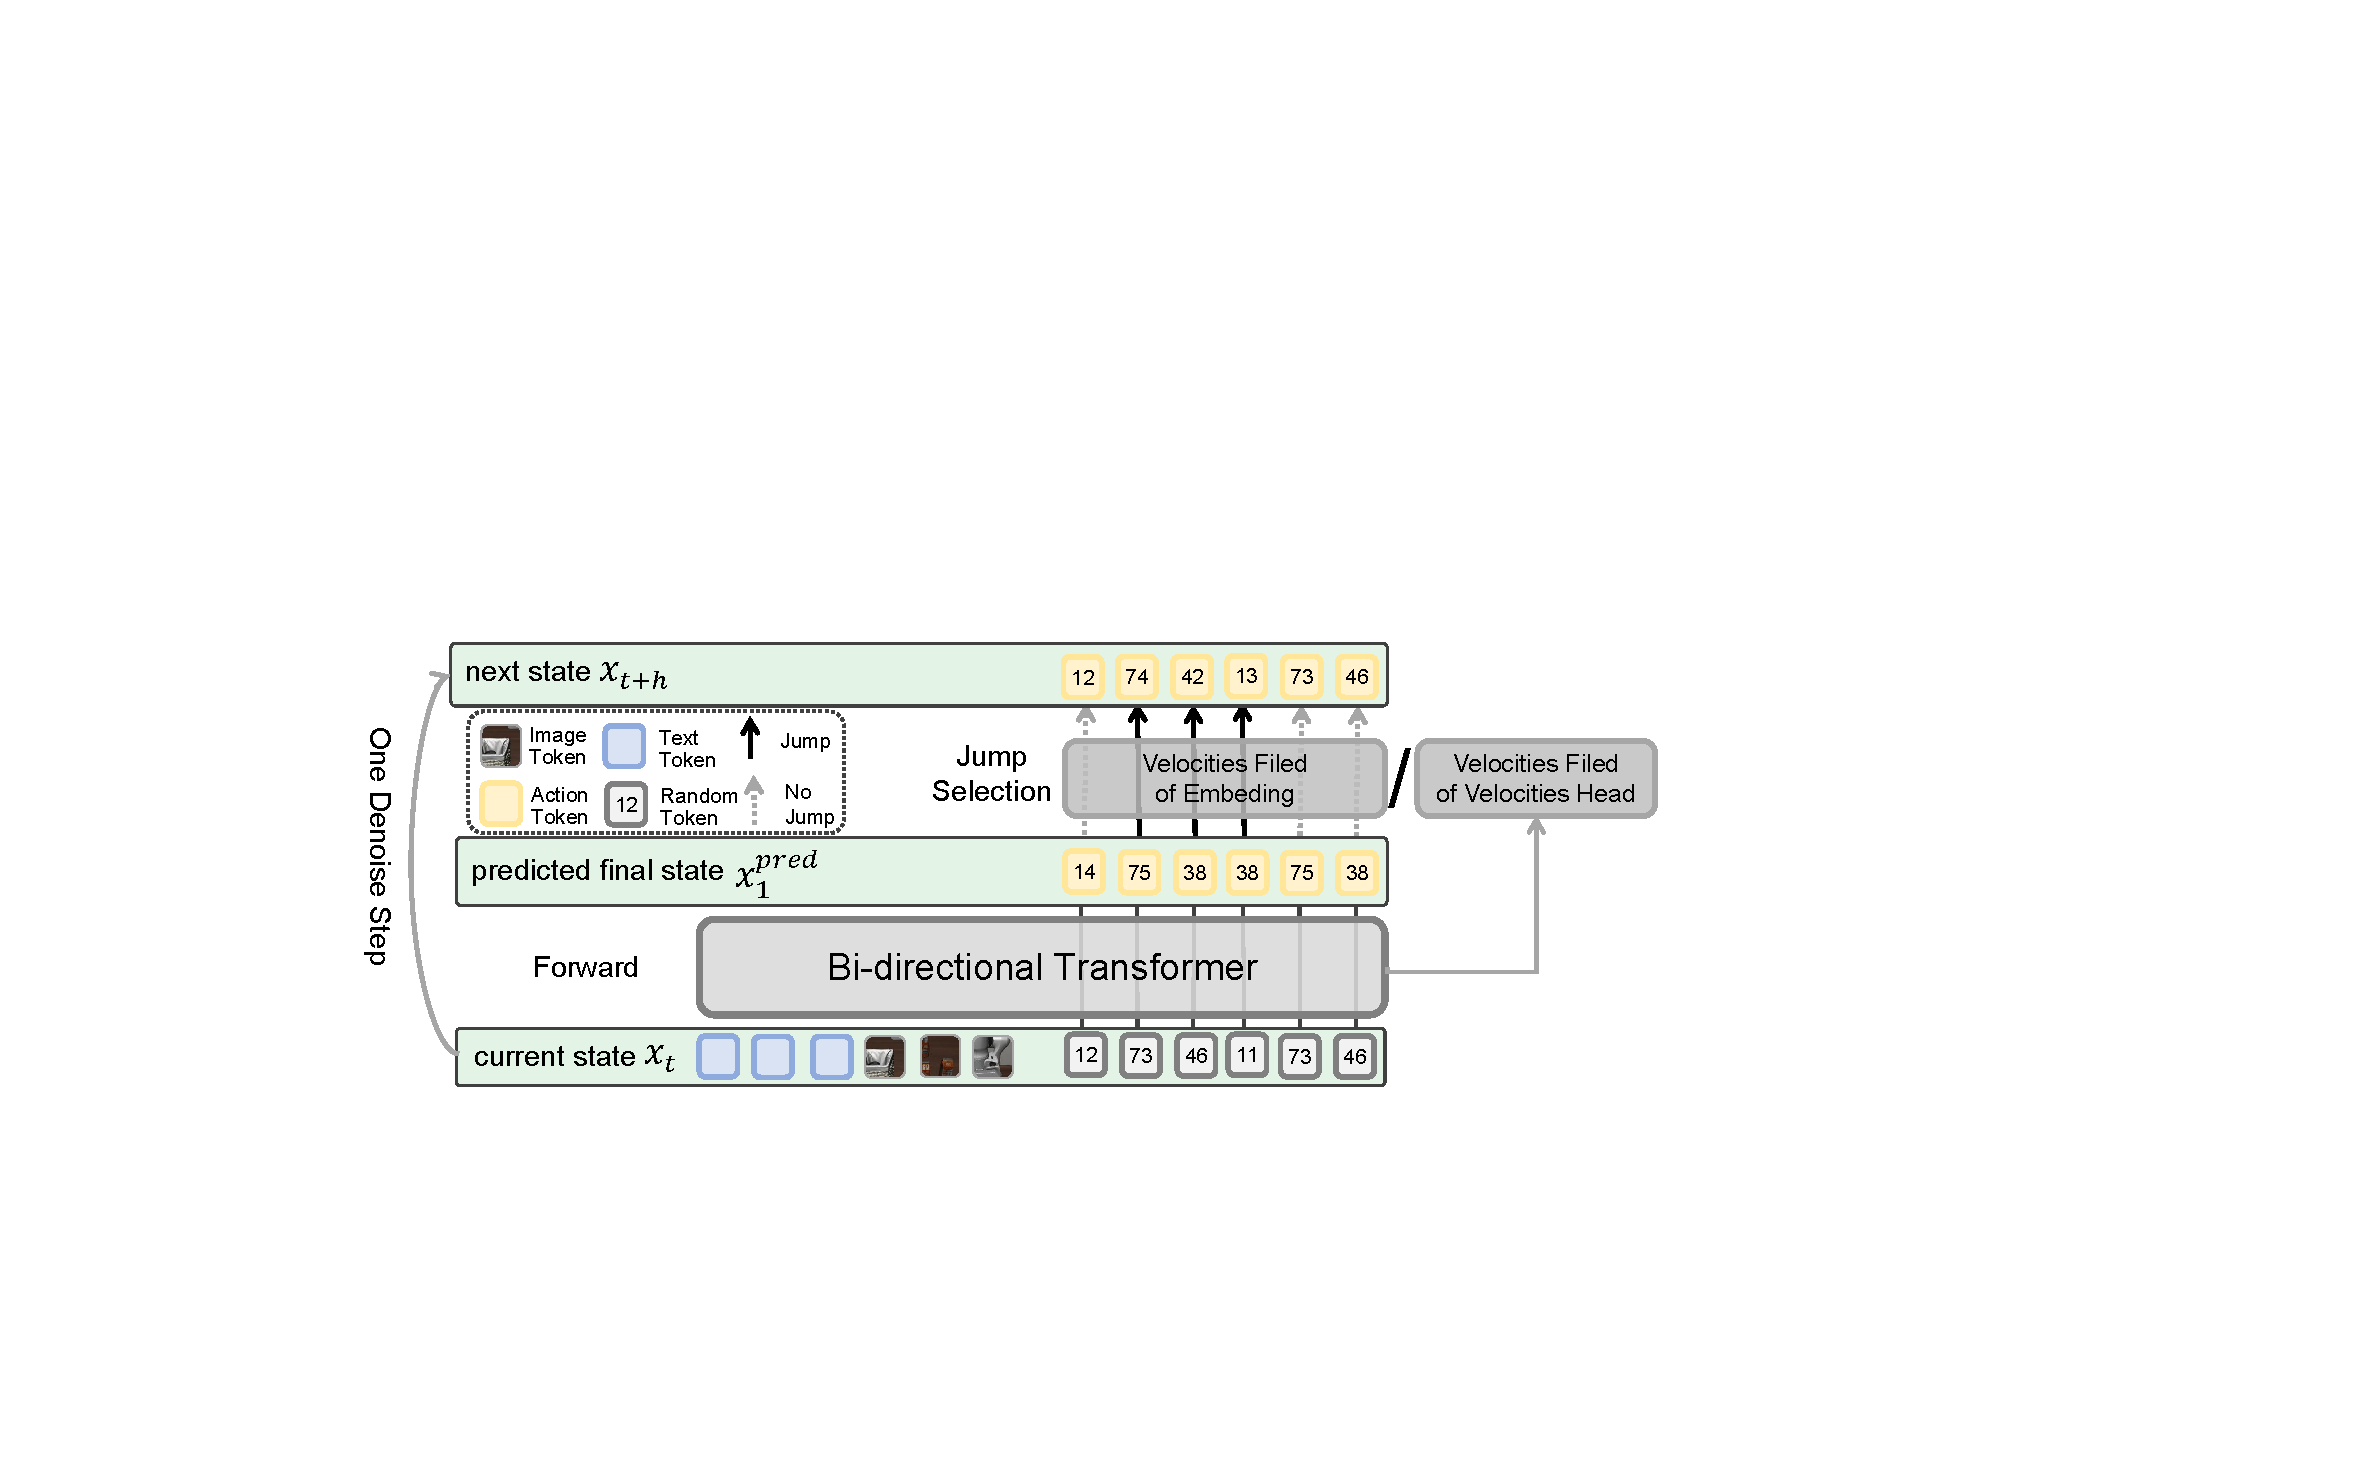
\includegraphics[width=0.98\linewidth]{figure/inference_one_step.pdf} 
    \caption{Visualization of a single decoding step in the iterative refinement stage. After predicting final state $x^\text{pred}_1$, the model does not directly output final action tokens. Instead, it constructs a velocity field to compute transition rates and selectively updates tokens to next state $x_{t+h}$ at each step.}
    \label{fig:inference} 
\end{figure*}
We perform inference in two stages: an iterative refinement stage followed by a deterministic validation stage, with $T_{\mathrm{fine}}$ and $T_{\mathrm{val}}$ decoding steps, respectively.

In the iterative refinement stage, we employ an Euler discretization of the continuous-time Markov chain (CTMC) process \( (x_t)_{0 \leq t \leq 1} \), following the approach in\citep{deng2025uniform}. As illustrated in \Cref{fig:inference}, for each coordinate \(i\) and each step from \(t\) to \(t+h\), we perform:
\begin{itemize}[itemsep=0pt, parsep=0pt, leftmargin=2em]
  \item Sample \( x_1^i \sim p_{1|t}^i(\cdot \mid x_t, l) \) from the model;
  \item Compute the total outgoing rate \( \lambda^i = \sum_{x^i \neq x_t^i} u_t^i(x^i, x_t^i \mid x_1^i) \) using Eq.~\ref{eq:ko-verlocity} or Eq.~\ref{eq:head-verlocity};
  \item Draw \( Z^i_{\text{change}} \sim U[0,1] \);
  \item Update \( x_{t+h}^i \): if \( Z^i_{\text{change}} \leq 1 - e^{-h\lambda^i} \), sample from \( \frac{u_t^i(\cdot, x_t^i \mid x_1^i)}{\lambda^i}(1-\delta_{x_t^i}(\cdot)) \); otherwise keep \( x_{t+h}^i=x_t^i \).
\end{itemize}
Here, \(\lambda^i\) is the total transition intensity out of the current token \(x_t^i\), so the jump probability \(1-e^{-h\lambda^i}\) increases with \(\lambda^i\). When a jump occurs, normalized rates favor states with larger velocity flow, which typically move the token closer to the predicted clean state \(x_1^i\). Repeating this process over time enables iterative correction across the full sequence.
Compared with mask-based discrete diffusion methods~\citep{yedreamVLA}, this decoding scheme allows previously updated tokens to be revised again in later iterations, rather than being permanently fixed after being predicted.
% \looseness=-1

\noindent
During the validation stage, we adopt a greedy decoding strategy to improve stability in the final refinement steps. 
In the final $T_{\mathrm{val}}$ decoding steps, we disable stochastic jumps and switch to greedy decoding,
\begin{equation}
    x_{t+h} = \arg\max \mathrm{softmax}(p_{1|t}(\cdot | x_t)),
\end{equation}
% where $\hat{y}_t$ is the model output logits. 
This hybrid design preserves exploratory refinement in earlier iterations while enforcing deterministic convergence near the end, leading to more stable validation-time trajectories and improved reproducibility. 
The concise two-stage decoding procedure is summarized in \Cref{alg:two_stage_sampling}.

\begin{algorithm}[b]
\caption{Two-Stage Decoding of \method}
\label{alg:two_stage_sampling}
\begin{algorithmic}[1]
\STATE \textbf{Input:} predictor $p_\theta$, context $l$, steps $T_{\mathrm{fine}},T_{\mathrm{val}}$, action vocabulary $\mathcal{V}$
\STATE Sample $x_0 \sim \mathrm{Uniform}(\mathcal{V})$; set $T \gets T_{\mathrm{fine}} + T_{\mathrm{val}}$
\FOR{$k=1$ to $T$}
    \STATE $t \gets (k-1)/T$, $h \gets 1/T$
    \STATE $\hat{x}_1 \sim p_\theta(\cdot \mid x_t, l)$
    \IF{$k \le T_{\mathrm{fine}}$}
        \STATE Compute velocity $u_t$ from $\hat{x}_1$ (Eq.~\ref{eq:ko-verlocity} or Eq.~\ref{eq:head-verlocity})
        \STATE Update $x_{t+h}$ by a  CTMC Euler step
    \ELSE
        \STATE Update $x_{t+h} \gets \arg\max p_\theta(\cdot \mid x_t, l)$
    \ENDIF
\ENDFOR
\STATE \textbf{Output:}  action sequence $x_1$
\end{algorithmic}
\end{algorithm}

\noindent
\textbf{Adaptive KV Caching.}
Following the dynamic caching strategy of FAST-dLLM~\citep{wu2025fast} on discrete diffusion decoding, we exploit the fact that many tokens exhibit only minor KV-state changes across iterative denoising steps of DFM. 
We keep the instruction and observation KV caches largely fixed throughout inference, while adaptively updating the action-side cache based on the cosine similarity between current and cached value features.
Combined with the parallel refinement of \method, this dynamic KV reuse yields a 2.4$\times$ latency speedup over autoregressive decoding while preserving task performance (see~\Cref{tab:efficiency_main}).


\begin{table*}[t]
    \footnotesize
    % \renewcommand{\arraystretch}{1.2}
    \setlength{\tabcolsep}{5pt}
    \centering
    \caption{\textbf{Comprehensive Evaluation of Long-Horizon Robotic Manipulation on the CALVIN Benchmark.} UniVLA$^{*}$ denotes the variant without historical frames for fair comparison.}
    \resizebox{\textwidth}{!}{%
    \begin{tabular}{l l c c c c c c}
        \toprule
        \multirow{2}{*}{\textbf{Method}}  & \multirow{2}{*}{\textbf{Task}} & \multicolumn{5}{c}{\textbf{Tasks Completed in a Row}} & \textbf{Avg. Len $\uparrow$} \\
        \cmidrule(lr){3-7}
        &  & 1 & 2 & 3 & 4 & 5 & \\
        \midrule
        MCIL~\citep{lynch2020language} & ABCD$\rightarrow$D &0.373 & 0.027 & 0.002 & 0.000 & 0.000 & 0.40\\
        RT-1~\citep{brohan2022rt}  & ABCD$\rightarrow$D & 0.844 & 0.617 & 0.438 & 0.323 & 0.227 & 2.45 \\
        Robo-Flamingo~\citep{li2024vision} & ABCD$\rightarrow$D & 0.964 & 0.896 & 0.824 & 0.740 & 0.660 & 4.09 \\
        Deer~\citep{yue2024deer} & ABCD$\rightarrow$D & 0.982 & 0.902 & 0.821 & 0.759 & 0.670 & 4.13 \\
        GR-1~\citep{wu2023unleashing}  & ABCD$\rightarrow$D & 0.949 & 0.896 & 0.844 & 0.789 & 0.731 & 4.21 \\
        ReconVLA~\citep{song2025reconvla}  & ABCD$\rightarrow$D & 0.980 & 0.900 & 0.845 & 0.785 & 0.705 &  4.23 \\
        UniVLA$^{*}$~\citep{univla}  & ABCD$\rightarrow$D & 0.948 & 0.906 & 0.862 & 0.834 & 0.690 & 4.26 \\
        MODE~\citep{reussefficient}  & ABCD$\rightarrow$D & 0.971 & 0.925 & 0.879 & 0.835 & 0.779 & 4.39 \\
        UP-VLA~\citep{zhang2025upvla}  & ABCD$\rightarrow$D & 0.962 & 0.921 & 0.879 & 0.842 & \textbf{0.812} & 4.42 \\
        % MDT~\citep{reuss2024multimodal}  & ABCD$\rightarrow$D & 0.986 & 0.958 & 0.916 & 0.862 & 0.801 & 4.52 \\
        % RoboVLMs~\citep{li2024towards} & ABCD$\rightarrow$D & 0.967 & 0.930 & 0.899 & 0.865 & 0.826 & 4.49 \\
        \rowcolor[gray]{0.9} \textbf{\method+Head}  & ABCD$\rightarrow$D & 0.968 & 0.928 & 0.880 & \textbf{0.864} & 0.776 & 4.42\\
        \rowcolor[gray]{0.9} \textbf{\method+Embed}  & ABCD$\rightarrow$D & \textbf{0.976} & \textbf{0.944} & \textbf{0.892} & 0.844 & 0.780 & \textbf{4.44}\\

        \bottomrule
    \end{tabular}
    }
    \label{tab:calvin_results}
    \vspace{-0.3cm}

\end{table*}
\begin{table*}[t]
\setlength{\tabcolsep}{10pt}
\footnotesize
\centering
\caption{\textbf{Evaluation and comparison on the LIBERO benchmark.}}
\resizebox{\textwidth}{!}{%
\begin{tabular}{lcccc|c}
\toprule
\textbf{Method} & \textbf{Spatial} & \textbf{Object} & \textbf{Goal} & \textbf{Long} & \textbf{Average} \\
\midrule
% DP*~\citep{chi2023diffusion}         & 78.3\% & 92.5\% & 68.3\% & 50.5\% & 72.4\% \\
Octo~\citep{octo_2023}               & 78.9\% & 85.7\% & 84.6\% & 51.1\% & 75.1\% \\
% OpenVLA~\citep{kim2024openvla}       & 84.9\% & 88.4\% & 79.2\% & 53.7\% & 76.5\% \\
SpatialVLA~\citep{qu2025spatialvla}  & 88.2\% & 89.9\% & 78.6\% & 55.5\% & 78.1\% \\
CoT-VLA~\citep{zhao2025cot}          & 87.5\% & 91.6\% & 87.6\% & 69.0\% & 81.1\%\\
WorldVLA~\citep{worldvla}          & 87.6\% &  96.2\% & 83.4\% & 60.0\% & 81.8\%\\
ThinkAct~\citep{huang2025thinkact}          & 88.3\% &  91.4\% & 87.1\% & 70.9\% & 84.4\%\\
$\pi_0$-FAST~\citep{pertsch2025fast} & 96.4\% & 96.8\% & 88.6\% & 60.2\% & 85.5\% \\
MolmoAct~\citep{lee2025molmoact}          & 87.0\% &  95.4\% & 87.6\% & 77.2\% & 86.6\%\\
FlowVLA~\citep{zhong2025flowvla}          & 93.2\% &  95.0\% & 91.6\% & 72.6\% & 88.1\%\\
DreamVLA~\citep{dreamvla25}          & \textbf{97.5\%} &  94.0\% & 89.5\% & 89.5\% & 92.6\%\\
% OpenVLA-OFT~\citep{kim2024openvla}       & 96.2\% & 98.3\% & 96.2\% & 90.7\% & 95.3\% \\
% UniVLA~\citep{univla}          & 95.4\% &  98.8\% & 93.6\% & 94.0\% & 95.5\%\\
% F1~\citep{f1_vla_2025}          & \textbf{98.2}\% &  97.8\% & \textbf{95.4}\% & 91.3\% & 95.7\%\\
% \rowcolor[gray]{0.9} \textbf{\method} & 96.2\% & \textbf{98.8\%} & 94.2\% & \textbf{95.2\%} & \textbf{96.1\%}\\
\rowcolor[gray]{0.9} \textbf{\method+Head} & 94.2\% & 96.4\% & 92.8\% & 90.4\% & 93.5\% \\
\rowcolor[gray]{0.9} \textbf{\method+Embed} & 96.8\% & \textbf{98.8\%} & \textbf{94.4\%} & \textbf{92.6\%} & \textbf{95.7\%}\\
\bottomrule
\end{tabular}
}
\label{tab:libero}
\vspace{-3mm}
\end{table*}


